\chapter{Grafy}

Pro tvorbu grafů v \LaTeX{}u je běžně používaný balíček \texttt{tikz}. Tento balíček poskytuje velmi flexibilní a výkonný nástroj pro kreslení grafů a diagramů. Pro specifické případy, jako je kreslení datových grafů, se však často využívá balíček \texttt{pgfplots}, který je postaven na \texttt{tikz} a poskytuje uživatelsky přívětivější rozhraní. \texttt{pgfplots} podporuje různé typy grafů, jako jsou sloupcové grafy, čárové grafy, spojnicové grafy, histogramy a další.

\section{Bar Chart (Sloupcový graf)}

Sloupcový graf je jednoduchý typ grafu, který slouží k zobrazení kategoriálních dat. V následujících příkladech ukazujeme, jak vytvořit sloupcový graf pomocí \texttt{pgfplots}.

\subsection{Základní Bar Chart}
\begin{chart}[H]
    \centering
    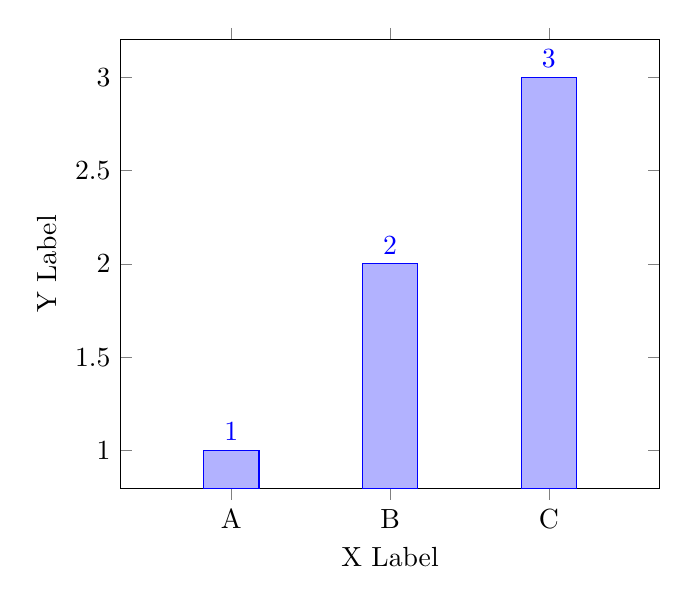
\begin{tikzpicture}
        \begin{axis}[ 
            xlabel={X Label},
            ylabel={Y Label},
            ybar, 
            xtick={1,2,3}, 
            bar width=20pt,
            nodes near coords, % Zobrazuje hodnoty přímo nad sloupci
            symbolic x coords={A, B, C}, % Popisky na ose x
            xtick=data,
            enlarge x limits=0.35 % Reduce the space on the x-axis
        ]
            \addplot coordinates {(A, 1) (B, 2) (C, 3)};
        \end{axis}
    \end{tikzpicture}
    \caption{Jednoduchý sloupcový graf}
    \label{chart:bar}
\end{chart}

\subsection{Sloupcový graf s více sadami dat}
\begin{chart}[H]
    \centering
    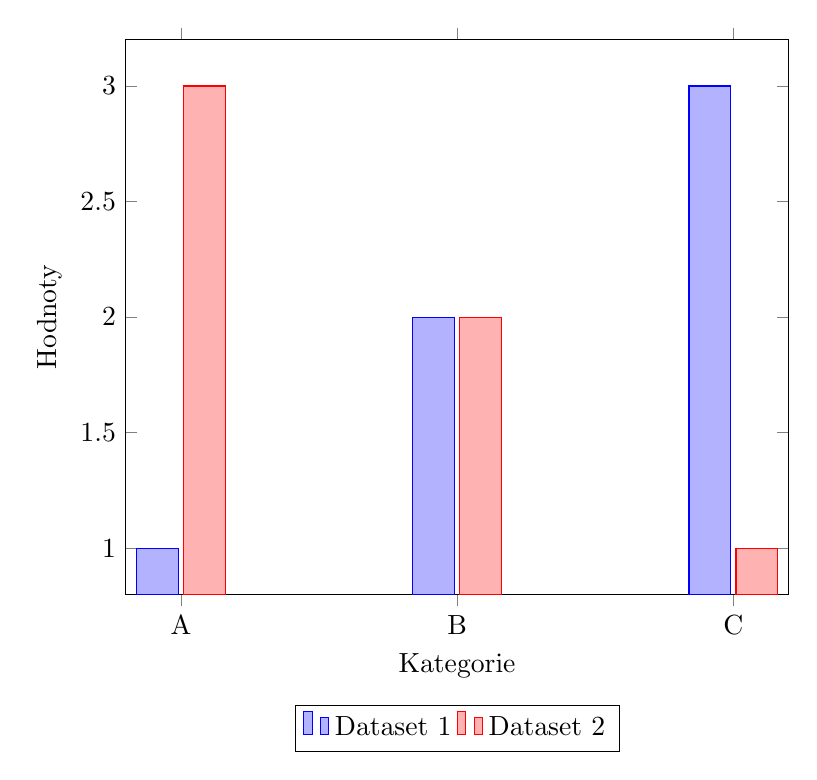
\begin{tikzpicture}
        \begin{axis}[
            ybar,
            xtick=data,
            bar width=15pt,
            width=10cm,
            xlabel={Kategorie},
            ylabel={Hodnoty},
            legend style={at={(0.5,-0.2)}, anchor=north, legend columns=-1},
            symbolic x coords={A, B, C},
            xtick=data
        ]
            \addplot coordinates {(A, 1) (B, 2) (C, 3)};
            \addplot coordinates {(A, 3) (B, 2) (C, 1)};
            \legend{Dataset 1, Dataset 2}
        \end{axis}
    \end{tikzpicture}
    \caption{Sloupcový graf se dvěma datovými sadami}
    \label{chart:bar2}
\end{chart}

\section{Stacked Bar Chart (Skládaný sloupcový graf)}

Skládaný sloupcový graf se používá k zobrazení kumulativních hodnot různých kategorií. Následující příklad ukazuje, jak lze vytvořit skládaný sloupcový graf:

\begin{chart}[H]
    \centering
    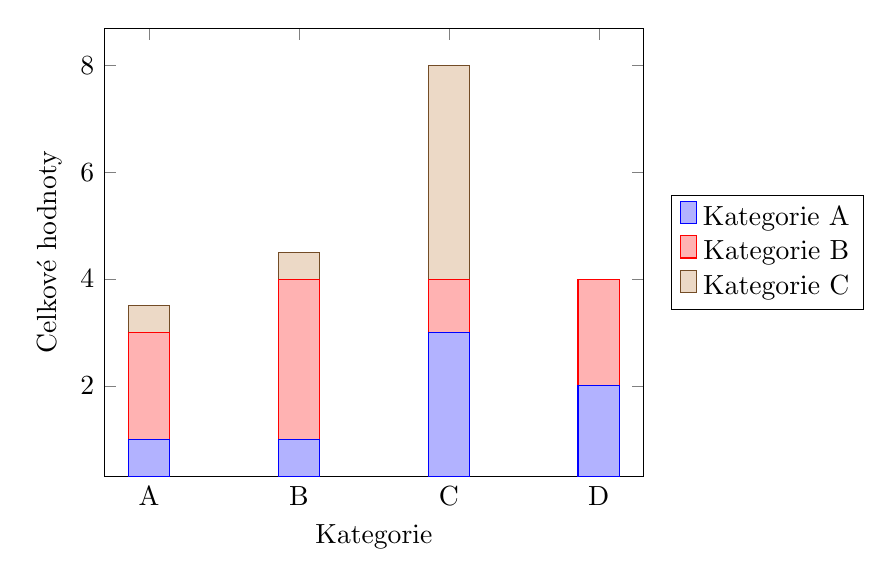
\begin{tikzpicture}
        \begin{axis}[
            ybar stacked,
            xlabel={Kategorie},
            ylabel={Celkové hodnoty},
            legend style={at={(1.05,0.5)}, anchor=west},
            symbolic x coords={A, B, C, D},
            xtick=data,
            bar width=15pt
        ]
            \addplot coordinates {(A,1) (B,1) (C,3) (D,2)};
            \addplot coordinates {(A,2) (B,3) (C,1) (D,2)};
            \addplot coordinates {(A,0.5) (B,0.5) (C,4) (D,0)};
            \legend{Kategorie A, Kategorie B, Kategorie C}
        \end{axis}
    \end{tikzpicture}
    \caption{Skládaný sloupcový graf}
    \label{chart:stacked}
\end{chart}

\section{Line Chart (Čárový graf)}

Čárový graf je vhodný pro zobrazení trendů v datech v čase nebo na kontinuální ose.

\begin{chart}[H]
    \centering
    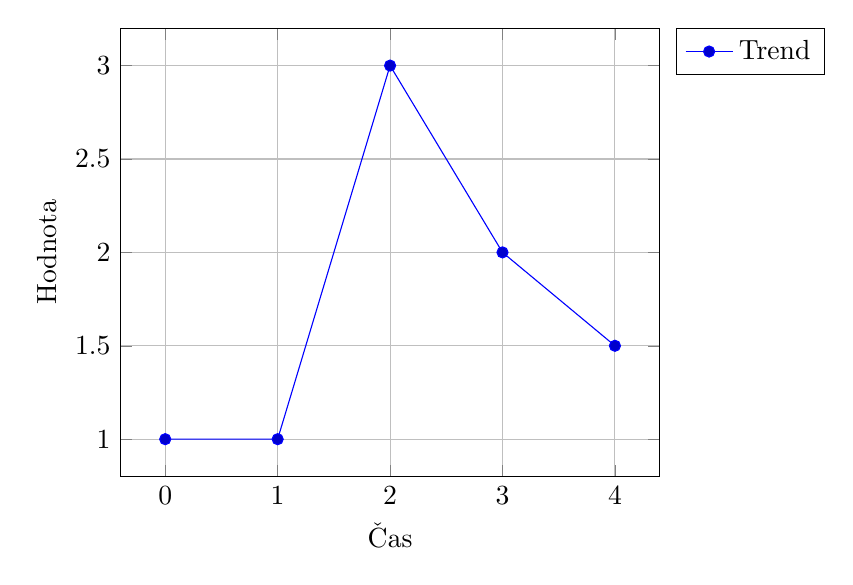
\begin{tikzpicture}
        \begin{axis}[
            xlabel={Čas},
            ylabel={Hodnota},
            grid=major, % Zobrazení mřížky
            legend pos=outer north east
        ]
            \addplot coordinates {(0,1) (1,1) (2,3) (3,2) (4,1.5)};
            \legend{Trend}
        \end{axis}
    \end{tikzpicture}
    \caption{Čárový graf ukazující trend}
    \label{chart:line}
\end{chart}

\section{Area Chart (Plošný graf)}

Plošný graf je varianta čárového grafu, kde je plocha pod křivkou vyplněna.

\begin{chart}[H]
    \centering
    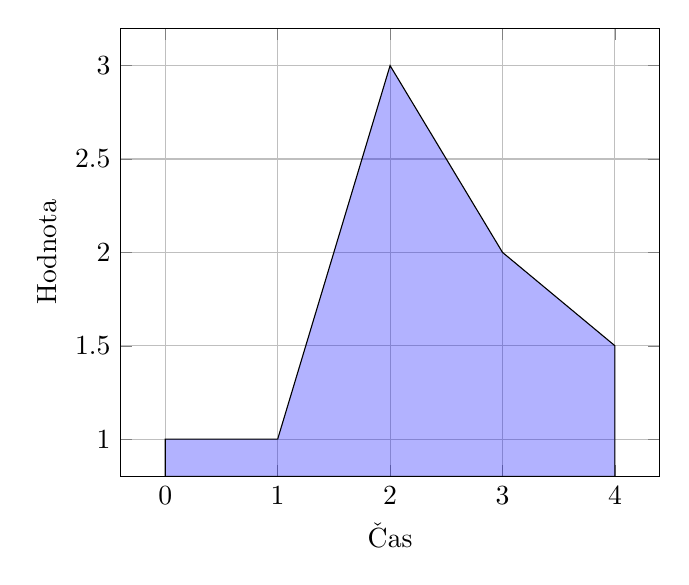
\begin{tikzpicture}
        \begin{axis}[
            xlabel={Čas},
            ylabel={Hodnota},
            grid=major,
        ]
            \addplot[fill=blue, fill opacity=0.3] coordinates {(0,1) (1,1) (2,3) (3,2) (4,1.5)} \closedcycle;
        \end{axis}
    \end{tikzpicture}
    \caption{Plošný graf}
    \label{chart:area}
\end{chart}

\section{Scatter Plot (Bodový graf)}

Bodový graf slouží k zobrazení vztahů mezi dvěma proměnnými.

\begin{chart}[H]
    \centering
    \begin{tikzpicture}
        \begin{axis}[scatter/classes={a={mark=square*,blue}, b={mark=triangle*,red}, c={mark=o,draw=black}},
            xlabel={Proměnná X},
            ylabel={Proměnná Y}]
            \addplot[scatter,only marks,scatter src=explicit symbolic]
            coordinates {
                (0.1,0.15) [a]
                (0.45,0.27) [c]
                (0.02,0.17) [a]
                (0.06,0.1) [a]
                (0.9,0.5) [b]
                (0.5,0.3) [c]
                (0.85,0.52) [b]
                (0.12,0.05) [a]
                (0.73,0.45) [b]
                (0.53,0.25) [c]
                (0.76,0.5) [b]
                (0.55,0.32) [c]
            };
        \end{axis}
    \end{tikzpicture}
    \caption{Bodový graf}
    \label{chart:scatter}
\end{chart}

\section{Pie Chart (Koláčový graf)}

Koláčový graf se používá k zobrazení podílů jednotlivých částí na celku.

\begin{chart}[H]
    \centering
    \begin{tikzpicture}
        \pie{10/A, 20/B, 30/C, 40/D}
    \end{tikzpicture}
    \caption{Koláčový graf}
    \label{chart:pie}
\end{chart}

\section{Histogram}

Histogram je vhodný pro zobrazení distribuce dat.

\begin{chart}[H]
    \centering
    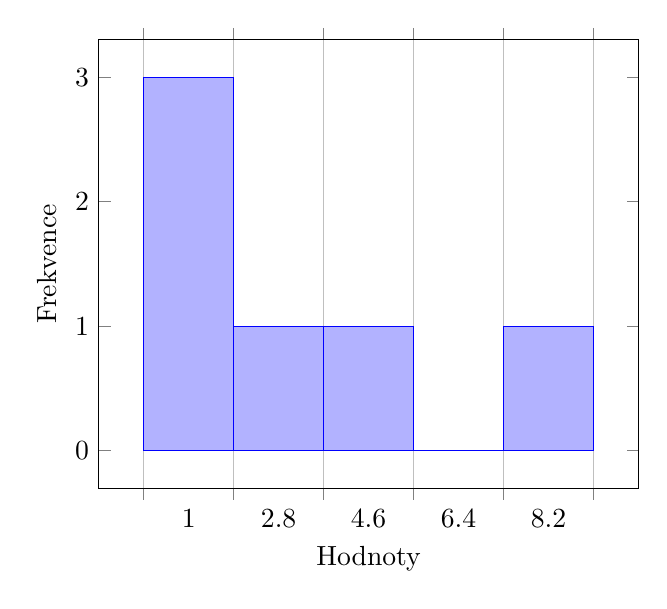
\begin{tikzpicture}
        \begin{axis}[
            ybar interval,
            xlabel={Hodnoty},
            ylabel={Frekvence}
        ]
            \addplot+[hist={bins=5}]
            table[row sep=\\,y index=0] {
                data\\
                1\\ 2\\ 1\\ 5\\ 4\\ 10\\
            };
        \end{axis}
    \end{tikzpicture}
    \caption{Histogram distribuce dat}
    \label{chart:histogram}
\end{chart}
